\documentclass{article}
\usepackage{amsmath}
\usepackage{amsfonts}
\usepackage{amssymb}
\usepackage{graphicx}
\usepackage[parfill]{parskip}
\usepackage{matlab-prettifier}
\usepackage{listings}
\usepackage{xcolor}
\usepackage{esvect}
\usepackage{mathtools}
\usepackage[a4paper, margin=2.54cm]{geometry}
\usepackage{float}

\title{MCEN 5228: Advanced Dynamics

HW4}
\author{David Akre}
\date{\today}

\begin{document}

\maketitle

\section{For the beam-spring system shown below, calculate the work done by gravity and the work done by the spring force on the beam length L as it rotates from the initial position of $\theta = 0^\circ$ to a position $\theta=90^\circ$ clockwise. Assume the beam has a mass $m$ and the spring behaves linearly with spring constant $k$. Also assume the unstretched length of the spring is $R$.}

\begin{figure}[H]
    \centering
    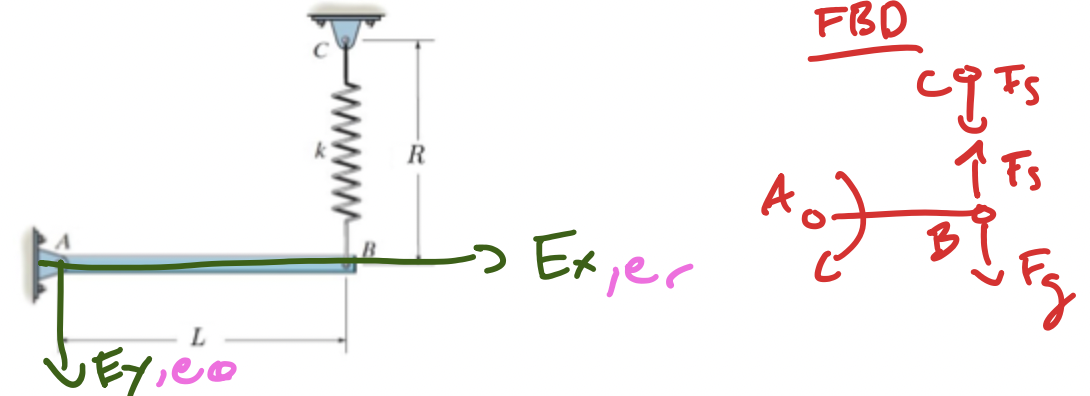
\includegraphics[width=0.6\linewidth]{problem1.png}
    \caption{Annotated Beam-Spring System}
\end{figure}

In the image above I have defined two coordinate systems one fixed in the inertial frame $\{E_x, E_y\}$ and another frame $\{e_r, e_{\theta}\}$ attached to point $B$ aligned to the spring  $\prescript{B}{}{\vv{r}}^{\, C}$.

Next the forces in this problem are represented to the right as a Free Body Diagram denoting one spring force and the gravitational force both acting on point $B$. These forces are:
\begin{align*}
    & F_g^B = m g E_y \\
    & F_s^B = -k \Delta \theta e_{\theta}
\end{align*}
Note $\Delta \theta$ is the displacement of the spring projected in the polar body coordinates. This can be transformed to the fixed inertial frame by noting $\Delta \theta$ is the arclength the beam travels relative to the unstretched position $R$ of the spring (i.e., $\prescript{A}{}{\vv{r}}^{\, B}$).
\begin{align*}
    & F_s^B = -k [2 \pi L \frac{\theta}{360^{\circ}} + R](\sin(\theta) E_x + \cos(\theta) E_y)
\end{align*}
Intuitively this makes sense as the spring force will act equal and opposite to the force of gravity in equilibrium as shown below.
\begin{align*}
    & \sum F_i = m_i a_i \text{ we're in equilibrium so } m_i a_i = \underbar{0} \\
    & \sum F_i = F_g^B + F_s^B = mg E_y - k R E_y = \underbar{0}
\end{align*}
The forces right now in the system are expressed in the fixed inertial frame, so the next step to calculate the virtual work done is to define the virtual displacements of the system (note we have 2 coordinates currently with 1 constraint on the beam so the minimial set of coordinates is simply $\theta$).
\begin{align*}
    & \delta \prescript{A}{}{\vv{r}}^{\, B} = \frac{d r}{d \theta} \delta \theta \\
    & \prescript{A}{}{\vv{r}}^{\, B} = [L - L \cos(\theta)] E_x + [L \sin(\theta)] E_y \\
    & \delta \prescript{A}{}{\vv{r}}^{\, B} = L * \delta \theta [\sin (\theta) E_x + \cos(\theta) E_y]
\end{align*}
The formula for virtual work is $\delta W = <F_i, \delta r_i>$ so the work done by gravity on the beam-spring system is:
\begin{align*}
    & \underline{\delta W_g = F_g \cdot \delta \prescript{A}{}{\vv{r}}^{\, B} = -m g L \cos(\theta) \delta \theta}
\end{align*}
The work done by the spring force is the following (let $S(\theta) = -k [2 \pi L \frac{\theta}{360^{\circ}} + R]$):
\begin{align*}
    & \delta W_s = F_s \cdot \delta \prescript{A}{}{\vv{r}^{\, B}} = L * \delta \theta * S(\theta) [\sin^2(\theta) + \cos^2(\theta)] \\
    & \underline{\delta W_s = L * \delta \theta * S(\theta)}
\end{align*}
Total work is now:
\begin{align*}
    & \delta W = \delta \theta * L(S(\theta) - m g \cos(\theta)) = 0 \\
    & \underline{S(\theta) = m g \cos(\theta)}
\end{align*}
Which confirms the prior formulation of the sum of forces acting on point $B$ of the system in equilibrium. Now to go from virtual work to total work done by the forces during infinitesimal virtual displacement we need to integrate over the generalized coordinate ($\theta$ from $0^{\circ} \to 90^{\circ}$ or $0 \to \pi/2$ radians which would imply $S(\theta) \to -k (r * \theta + R)$ simply.
\begin{align*}
    & \underline{W_g} = \int_{0}^{\pi/2} -m g L \cos(\theta) d\theta = -m g L (\sin(\theta))\Big|_0^{\pi/2} = -m g L (1 - 0) = \underline{-m g L} \\
    & \underline{W_s} = \int_{0}^{\pi/2} L S(\theta) d\theta = -L k [r \frac{\theta^2}{2} + R \theta]\Big|_0^{\pi/2} = \underline{-L k [L * \frac{\pi^2}{8} + R \frac{\pi}{2}]} \\
    & W_g + W_s = 0 \to \underline{m g = k [\frac{\pi^2}{8} + \frac{R \pi}{2 L}]}
\end{align*}

\section{The work-energy principle says that the work done by all external forces on a particle or rigid body is equal to the change in kinetic energy that it $W_{1 \to 2} = \Delta T$, where $T$ is the kinetic energy. Show that if the work term is broken up into the work done by conservative forces and the work done by non-conservative forces, $W_{1 \to 2} = W_{1 \to 2}^C + W_{1 \to 2}^{NC}$, then the work-energy principle becomes $W_{1 \to 2}^{NC} = \Delta T + \Delta V$. Also, show that if the work done by non-conservative forces acting the on the system $W_{1 \to 2}^{NC} = 0$, then the system energy $E = T + V$ is conserved between the initial and final states.}

The first part of the question asks us to show that if the work term is broken up into: $W_{1 \to 2} = W_{1 \to 2}^C + W_{1 \to 2}^{NC}$ then the work energy principle becomes $W_{1 \to 2}^{NC} = \Delta T + \Delta V$. In class it was shown that we can first transform coordinates to generalized coordinates $\{q_i\}$, then reformulate D'Alembert's Principle w.r.t T and V, and then as non-conservative external forces. So I'll show these steps and derivations to arrive at the final step used to show the equivalence in the statement the problem asks us to show.

The first step simply transforms coordinates that are dependent to a set of independent generalized coordinates (similar to problem 1 and 4).
\begin{align*}
    & \{r_i, i = 1, ..., N\} \to \{q_j, j = 1,..., n\} \text{ by the coordinate transformation below } \\
    & r_i = r_i(q_i, ..., q_n, t) \quad i \in [1, ..., N]
\end{align*}
The velocities w.r.t to the generalized coordinates are the following:
\begin{align*}
    & v_i = \sum_i^n \frac{\partial r_i}{\partial q_j} \dot{q}_j + \frac{\partial r_i}{dt} 
\end{align*}
Which leads to the following equivalence statement when taking the partial derivative of the above w.r.t. $\dot{q}_j$:
\begin{align*}
    & \frac{\partial v_i}{\partial \dot{q}_g} = \frac{\partial r_i}{\partial q_i} \quad i \in [1, ..., N], j \in [1, ..., n]
\end{align*}
Likewise virtual displacement are:
\begin{align*}
    & \delta r_i = \sum_j^n \frac{\partial r_i}{\partial q_j} \delta q_j \quad i \in [1, ..., N]
\end{align*}
So from D'Alembert's Principle we arrive at:
\begin{align*}
    & \sum_i^N <F_i, m_i \ddot{r}_i, \delta r_i> = 0 \\
    & \sum_i^N <F_i, \delta r_i> - \sum_i^N<m_i \ddot{r}_i, \delta r_i> = 0
\end{align*}
Where the left summand is the virtual work due to external forces and the right is the virtual work due to inertial forces. Next step is to reformulate this into terms of kinetic and potential energy (T and V) leveraging properties of inner product spaces linearity, symmetry, and product rules. Starting with the virtual work due to inertial force.
\begin{align*}
    & \sum_i^N <m_i \ddot{r}_i, \delta r_i> = \sum_i^N <m_i \ddot{r}_i, \sum_j^n \frac{\partial r_i}{\partial q_j} \delta q_j> = \sum_i^N \sum_j^n \underline{<m_i \ddot{r}_i, \frac{\partial r_i}{\partial q_j}> \delta q_j} \text{ focusing on this part} \\
    & <m_i \ddot{r}_i, \frac{\partial r_i}{\partial q_j}> = <\frac{d}{dt}(m_i \dot{r}_i), \frac{\partial r_i}{\partial q_j} \to \underline{\frac{d}{dt}<m_i \dot{r}_i, \frac{\partial r_i}{\partial q_j}>} - <m_i \dot{r}_i, \underline{\frac{d(\partial r_i)}{dt(\partial q_j)}}> \\
    & \text{First part } \frac{\partial}{\partial \dot{q}_j}<m_i v_i, v_i> = <\frac{\partial}{\partial \dot{q}_j}(m_i v_i), v_i> + <m_i v_i, \frac{\partial v_i}{\partial \dot{q}_j}> = m_i <\frac{\partial v_i}{\dot{q}_j},v_i> + <m_i, \frac{\partial v_i}{\partial \dot{q}_j}> \\
    & = 2 <m_i v_i, \frac{\partial v_i}{\partial \dot{q}_j}>  \\
    & \text{Second part }\frac{d(\partial r_i)}{dt(\partial q_j)} = \frac{\partial v_i}{\partial q_j} \\
    & \text{Altogether } \frac{\partial}{2 \partial \dot{q}_j} <m_i v_i, v_i> = \frac{\partial}{\partial \dot{q}_j}T_i
\end{align*}
Thus we arrive at the virtual work done by inertial forces via kinetic energy:
\begin{align*}
    & <m_i \ddot{r}_i, \frac{\partial r_i}{\partial q_j}> = \frac{d(\partial T_i)}{dt(\partial \dot{q}_j)} - \frac{\partial T_i}{\partial q_j}
\end{align*}
To solve for the total kinetic energy of the system we then simply plug the inertial kinetic energy back into D'Alembert's principle of virtual work equation from earlier.
\begin{align*}
    & \sum_i^N \sum_j^n <m_i \ddot{r}_i, \frac{\partial r_i}{\partial q_j}> \delta q_j \to \sum_i^N \sum_j^n[\frac{d(\partial T_i)}{dt(\partial \dot{q}_j)} - \frac{\partial T_i}{\partial q_j}] \delta q_j \\
    & \sum_j^n [\frac{d}{dt}[\frac{\partial}{\partial \dot{q}_j}(\sum_i^N T_i) - \frac{\partial}{\partial q_j}(\sum_i^N T_i)]]\delta q_j
\end{align*}
Now focusing in on the virtual work of the external / applied forces we have the following:
\begin{align*}
    & \sum_i^N <F_i, \delta r_i> \text{ where } \delta r_i = \sum_j^n \frac{\partial r_i}{\partial q_j}\delta q_j \\
    & \sum_i^N <F_i, \sum_j^n \frac{\partial r_i}{\partial q_j} \delta q_j> \to \sum_j^n \underline{\sum_i^N <F_i, \frac{\partial r_i}{\partial q_j}>} \delta q_j \\
    & Q_j = \sum_i^N <F_i, \frac{\partial r_i}{\partial q_j}> \quad j \in [1, ..., n]
\end{align*}
Where $Q_j$ are the generalized forces and putting this altogether now we have the following expression:
\begin{align*}
    & \sum_i^N <F_i, \delta r_i> - \sum_i^N <m_i \ddot{r}_i, \delta r_i> = \sum_j^n[Q_j - [\frac{d(\partial T)}{dt(\partial \dot{q}_j)} - \frac{\partial T}{\partial q_j}]] \delta q_j = 0
\end{align*}
The last step of the derivation is to split the conservative forces from the non-conservative ones from $Q_j$ noting that the work done by a conservative force is the difference in potential energy and its force is the negative gradient of a scalar potential (i.e., $F_i^C = -\nabla v_i$). So breaking out the forces into conservative and non-conservative we can arrive at the following virtual work expression:
\begin{align*}
    & \sum_i^N <F_i^{NC} + F_i^C, \delta r_i> = \sum_i^N <F_i^{NC}, \delta r_i> + \sum_i^N <F_i^C, \delta r_i> \\
    & \sum_j^n Q_j^{NC} \delta q_j + \sum_i^N - \delta v_i \to \sum_j^n Q_j^{NC} \delta q_j - \delta V \\
    & \sum_j^n \underline{(Q_j^{NC} - \frac{\partial V}{\partial q_j})} \delta q_j \text{ underline is } Q_j \\
    & \underline{\sum_j^n[(Q_j^{NC} - \frac{\partial V}{\partial q_j}) - \frac{d(\partial T)}{dt(\partial \dot{q}_j)} - \frac{\partial T}{\partial q_j}] \delta q_j = 0}
\end{align*}
So now to show that $W_{1 \to 2} = \Delta T + \Delta U$:
\begin{align*}
    & \delta W_{NC} = \sum_j^n Q_j^{NC} \delta q_j \\
    & \delta W_{C} = -\sum_j^n \frac{\partial V}{\partial q_j} \delta q_j = \delta V \\
    & \delta W_{T} = -\sum_j^n \frac{d(\partial T)}{dt(\partial \dot{q}_j)} + \frac{\partial T}{\partial q_j} \delta q_j \\
    & \underline{\delta W = \delta W_{NC} + \delta W_{C} + \delta W_{T} = 0}
\end{align*}
The above shows how the work can be borken up into parts of conservative, non-conservative, and inertial. Thus to show that $W_{1 \to 2}^{NC} = \Delta T + \Delta U$ is trivial since $W_{NC}$ is positive in the underlined section above, while $W_{C}$ + ${W_T}$ are negative thus showing that the work done by conservative and inertial forces balance with the non-conservative forces by further noting that $\delta q_j = \emptyset$ we are simply dealing with a balance of forces instead of virtual work.

So now if $W_{1 \to 2}^{NC} = 0$ and noting $\delta q_j = \emptyset$ this implies $Q_{NC} = 0$, and by property of balance of forces acting on a system in equilibrium the forces due to the inertial / kinetic will counteract against the conservative forces (i.e., $\sum F_C = m_i a_i = 0$). Thus the energy due to kinetic forces is $T = \frac{m v \cdot v}{2}$ and potential energy $V = -\int F_c dq_i$ result in $\underline{\underline{E = \frac{m v \cdot v}{2} - \int F_c dq_i = 0}}$ which follows the property of conservation of energy and noting that principle of virtual work is invariant to time (only subject by path and principle of least action).

\section{Consider the system shown in Problem 1. If this system starts at rest at the initial state $\theta = 0^\circ$, find the spring constant $k$ required such that the system is at rest in the final state $\theta = 90^{\circ}$ clockwise in terms of m, g, L, and R.}

Most of the work for this problem has been accomplished in 1 so we simply need to solve for $k$ now from the last step (equilibrium condition from work done from $0^\circ \to 90^\circ$)
\begin{align*}
    & mg = k(\frac{\pi^2}{8} + \frac{R \pi}{2 L}) \\
    & \underline{k = \frac{mg}{\frac{\pi2}{8} + \frac{R\pi}{2L}} = \frac{8 L mg}{\pi(\pi L + 4 R)}}
\end{align*}

\section{The system shown consists of a uniform rigid link of mass $m$ and length $L$ and the two springs with stiffness $k_1$ and $k_2$ respectively. When the springs are unstretched, the link is horizontal. Use the principle of virtual work to calculate the relationship between the angle $\theta$ and the parameters $k_1$, $k_2$, $m$, and $l$ at equilibrium.}

\begin{figure}[H]
    \centering
    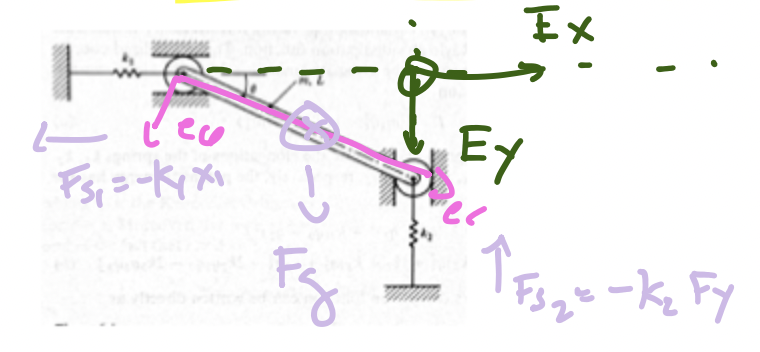
\includegraphics[width=0.6\linewidth]{problem4.png}
    \caption{Annotated Rigid Link System}
\end{figure}
In the annotated rigid system above I have defined two coordinate systems: one that is fixed in the inertial frame denoted as $\{E_x, E_y\}$ where the origin is where both springs are unstretched. The second coordinate system is defined along the rigid link as the body frame coordinate denoted as $\{e_r, e_{\theta}\}$.

Next the forces in the problem are represented on the diagram (i.e., two spring forces and one gravitational one). They are expressed below:
\begin{align*}
    & F_{s1} = -k_1 x E_x = -k_1(L - L \cos(\theta)) E_x \\
    & F_{s2} = -k_2 y E_y = -k_2 L \sin(\theta) E_y \\
    & F_g = m g \frac{L}{2} e_r 
\end{align*}
The last gravitational force is currently expressed in the body coordinate frame, so lets transform it into the fixed frame by the following:
\begin{align*}
    & \begin{bmatrix} E_x \\ E_y \end{bmatrix} = \begin{bmatrix} \cos(\theta) & -\sin(\theta) \\ \sin(\theta) & \cos(\theta) \end{bmatrix} \begin{bmatrix}e_r \\ e_{\theta}\end{bmatrix} \\
    & F_g = m g \frac{L}{2}[\cos(\theta) E_x + \sin(\theta) E_y]
\end{align*}
Since this is a statics problem, the sum of the forces is the following:
\begin{align*}
    & \sum F_i = m_i a_i \text{ where } m_i a_i = \underbar{0} \\
    & \sum F_i = F_x + F_y = \underbar{0} \\
    & F_x = -k_1 L (1 - \cos(\theta)) + m g \frac{L}{2} \cos(\theta) \\
    & F_y = -k_2 L \sin(\theta) + m g \frac{L}{2} \sin(\theta)
\end{align*}
The forces expressed in the inertial frame and group in the x and y directions respectively. The next step is to calculate the virtual displacements of the system where we have currently 2 coordinates with 1 constraint on the rigid link so the minimal set of coordinates can be reduced to just $\theta$ as shown below:
\begin{align*}
    & r_1 = x E_x \to \delta r_1 = \delta x E_x \\
    & r_2 = y E_y \to \delta r_2 = \delta y E_y \\
    & x = L - L \cos(\theta) \to \delta x = L \sin(\theta) \delta \theta \\
    & y = L \sin(\theta) \to \delta y = L \cos(\theta) \delta \theta
\end{align*}
We can finally calculate the virtual work of the system:
\begin{align*}
    & \delta W = \sum_i <F_i, r_i> = 0 \\
    & \delta W_x = F_x \cdot r_1 = [\underline{-k_1 L (1 - \cos(\theta)) + m g \frac{L}{2} \cos(\theta)}] L \sin(\theta) \delta \theta \\
    & \text{Let the underline section be a temporary variable A} \\
    & \delta W_y = F_y \cdot r_2 = [\underline{-k_2 L \sin(\theta) + m g \frac{L}{2} \sin(\theta)}] L \cos(\theta) \delta \theta \\
    & \text{Let the underline section be a temporary variable B} \\
    & \delta W = \delta W_x + \delta W_y = L \delta \theta [\sin(\theta) A + \cos(\theta) B] = 0 \\
    & -k_1 L \sin(\theta) + k_1 L \sin(\theta) \cos(\theta) + m g \frac{L}{2} \cos(\theta) \sin(\theta) - k_2 L \sin(\theta) \cos(\theta) + m g \frac{L}{2} \sin(\theta) \cos(\theta) \\
    & \sin(\theta) L [-k_1 + k_1 \cos(\theta) + \frac{m g}{2} \cos(\theta) - k_2 \cos(\theta) + \frac{m g}{2} \cos(\theta)] \\
    & \cos(\theta)(k_1 + m g - k_2) - k_1 = 0 \\
    & \cos(\theta) = \frac{k_1}{k_1 + m g - k_2} \\
    & \underline{\theta = \cos^{-1}(\frac{k_1}{k_1 + m g - k_2})}
\end{align*}

\end{document}